% !TEX encoding = UTF-8
% !TEX TS-program = pdflatex
% !TEX root = ../tesi.tex
% !TEX spellcheck = it-IT

%**************************************************************
\chapter{Conclusioni}
\label{cap:conclusioni}
%**************************************************************
\section{Consuntivo finale}
\label{consuntivo}
A differenza di quanto riportato dal calendario delle attività svolte durate lo stage, descritte nella \hyperref[calendario]{Sezione 3.2}, il piano di lavoro proposto inizialmente era molto generico definendo solamente delle fasi di massima in modo da lasciare spazio ad eventuali future modifiche o aggiunte:

\begin{enumerate}
\item \textbf{Settimana 1}: introduzione in azienda e condivisione \textit{password} aziendali;
\item \textbf{Settimana 2}: introduzione ai prodotti aziendali e condivisione manuali e documentazione riferiti ai prodotti di punta dell'azienda;
\item \textbf{Settimana 3}: formazione sui prodotti XE\footnotemark[1] e XC\footnotemark[1] legati alla fatturazione dell'energia elettrica;
\footnotetext[1]{Abbreviazioni dei prodotti XEnergy e XContract discussi nella \hyperref[prodotti]{Sezione 1.3}} 
\item \textbf{Settimana 4-5}: focalizzazione sul prodotto CSIndex ed esecuzione di test funzionali sulla nuova versione del \textit{software} (NPS EBS) in affiancamento al tutor;
\item \textbf{Settimana 6-7}: manualistica, U.A.T\footnotemark[2],
\footnotetext[2]{Test visti nella \hyperref[fasi progetto]{Sezione 1.4.2}} \textit{roll out} del progetto NPS EBS;
\item \textbf{Settimana 8}: verifica dell'apprendimento degli obiettivi prefissati.
\end{enumerate}

Per avere una visione d'insieme delle attività inizialmente pianificate, riporto il corrispondente \gls{diagramma di Gantt} nella \hyperref[gantt pianificazione]{Figura 4.1}.

\begin{figure}[h!]
\begin{center}
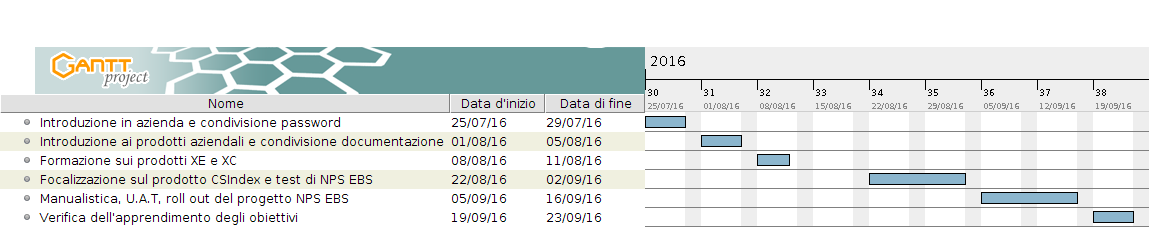
\includegraphics[scale=0.32]{GanttPianificazione} 
\caption{Diagramma di Gantt delle attività che erano state pianificate}
\label{gantt pianificazione}
\end{center}
\end{figure}
\FloatBarrier

\newpage
Le cause principali che hanno spinto a cambiare il piano di lavoro proposto, sono ricollegabili soprattutto al fatto che sono sorti dei rischi che non erano stati calcolati o per meglio dire delle situazioni imprevedibili come le dimissioni di una collega che risultava essere una delle figure di riferimento per alcuni clienti considerati molto importanti nel contesto aziendale. \\
Questo fatto ha attirato l'attenzione di tutto il personale proprio al momento del mio arrivo in Mediana S.r.l.u., con malumori dovuti a continue riunioni per effettuare imminenti e problematici passaggi di consegne del lavoro che la collega stava svolgendo per i progetti che in parte avrebbero dovuto coinvolgermi (XE e XC). \\
Per questo motivo il mio tutor ha giustamente preferito focalizzare il mio stage soltanto su NPS EBS, preferendo rimandare ad un possibile futuro la mia formazione sugli altri prodotti, sui quali mi è stata fatta solamente una breve panoramica. \\
Quindi essendo di fatto saltata la pianificazione della seconda e terza settimana ed essendo state largamente sovrastimate alcune fra le attività restanti, piuttosto che continuare a svolgere gli stessi incarichi, che iniziavano ad essere troppo ripetitivi e per questo non più molto istruttivi, ho deciso, in accordo con il tutor interno e il tutor aziendale, di cogliere l'opportunità di prendere un posto lasciato vacante da sviluppatore, come avevo già anticipato nella \hyperref[seconda fase]{Sezione 3.5}, non appena questo si è liberato. 

\section{Raggiungimento degli obiettivi}
Gli obiettivi che erano stati delineati sono da considerarsi quasi tutti superati, nonostante il cambiamento che c'è stato nella pianificazione. Infatti, trattandosi più che altro di un progetto formativo, gli obiettivi non erano del tutto concreti, ma fungevano più che altro da linea guida da seguire per riuscire ad essere introdotto al meglio nella realtà aziendale di Mediana S.r.l.u e nel lavoro da consulente dando allo stesso tempo uno sguardo ad un possibile futuro in questo ambito, tramite un inserimento nell'organico per un periodo più lungo delle canoniche 8 settimane di stage nel caso entrambi le parti fossero uscite da questa esperienza in maniera positiva.
Nella \hyperref[tabella obiettivi]{Tabella 4.1} riporto la lista degli obiettivi già visti nella \hyperref[obiettivi]{Sezione 1.1}, specificando per ognuno di essi le ragioni per le quali possano essere considerati come raggiunti o meno.

\newpage
\normalsize
\begin{longtable}{|>{\centering}m{6cm}|m{6cm}<{\centering}|}
\hline
\textbf{Obiettivo} & \textbf{Raggiungimento}\\
\hline
\endhead
{Conoscenza degli applicativi di Mediana S.r.l.u., in particolare di CSIndex nella sua ultima versione NPS EBS} & {\textbf{Parzialmente raggiunto}: a discapito di una più approfondita conoscenza del \textit{software} NPS EBS, che come spiegato più volte si rifà al più generico CSIndex, e a causa di un evento non prevedibile, come discusso nella \hyperref[consuntivo]{Sezione 4.1}, purtroppo è stata accantonata l'idea di farmi conoscere gli altri prodotti offerti da Mediana S.r.l.u.} 
\\ \hline

{Conoscenza delle fasi consulenziali come:
	\begin{itemize}
	\item Redazione di \textit{test book} per U.A.T.\footnotemark[1];
	\item Test e verifiche dei programmi presi in esame;
	\item Redazione di manuali propedeutici al \textit{roll out} dell'applicativo.
	\end{itemize}} & {\textbf{Interamente raggiunto}:  incarichi appresi tutti durante la prima metà dello stage, descritta nella \hyperref[prima fase]{Sezione 3.4}}
\\ \hline

{Apprendimento del \gls{data model} di NPS EBS} & {\textbf{Interamente raggiunto}: ho imparato a conoscere il \gls{data model} di NPS sia teoricamente durante la fase di test e stesura dei manuali, rispettivamente \hyperref[test]{Sezione 3.4.2} e \hyperref[manuali]{Sezione 3.4.3}, che più approfonditamente nella seconda metà dello stage, descritta nella \hyperref[seconda fase]{Sezione 3.5}, quando ho potuto mettere le mani al codice}
\\ \hline

{Sviluppare una buona autonomia nella progettazione e sviluppo di \textit{statement} SQL} & {\textbf{Interamente raggiunto}: in parte già presente nel mio bagaglio culturale poiché si tratta di una capacità che ho appreso durante il corso di Basi di Dati, è stata sicuramente rafforzata in base alle esigenze avute durante la seconda metà dello stage quando ho dovuto esplorare il database di NPS per risolvere alcuni bug, come ho descritto nella \hyperref[db]{Sezione 3.4.2}}
\\ \hline

\caption[Tabella Requisiti Implementati]{Tabella Requisiti Implementati}
\label{tabella obiettivi}
\end{longtable}

%**************************************************************
\newpage
\section{Conoscenze acquisite}
L'esperienza di stage effettuata ha contribuito sicuramente ad ampliare le mie conoscenze professionali. \\
In particolare avendo avuto l'occasione di provare, anche se solo in parte, gli impieghi di un consulente tecnico, sono riuscito a comprendere le dinamiche di un lavoro che prima di allora non avevo mai preso in considerazione. \\
Allo stesso tempo però il fatto di essere riuscito a occupare una parte di stage come sviluppatore, anche se soltanto effettuando semplici operazioni di \textit{bug-fixing}, mi ha permesso di arricchire le mie conoscenze informatiche con lo studio di tecnologie mai utilizzate in precedenza, come C\# e ASP.NET, delle quali ho già avuto modo di parlare nella \hyperref[tecnologie]{Sezione 1.5.2}. \\
Oltre alle conoscenze tecniche appena descritte, l'attività di stage mi ha
permesso soprattutto di entrare in ottica aziendale potendo così imparare a relazionarmi al meglio con i colleghi e a collaborare con loro per uno stesso obiettivo. \\
Prima di allora infatti non avevo mai avuto modo di misurare le mie capacità in ambito
lavorativo e grazie a quest'esperienza ho potuto notare, rispetto ai progetti svolti durante i corsi universitari, alcune nette differenze nella gestione di un progetto. Mi riferisco soprattutto al fatto che si tende a voler rilasciare un prodotto nel minor tempo possibile piuttosto che puntare ad avere una buona qualità ed affidabilità che si va invece ad ottenere man mano nel tempo attraverso lunghe fasi di \textit{support}. Ciò è dovuto probabilmente al fatto che esistono profonde differenze tra gli obiettivi che ci sono nel mondo del lavoro e quelli presenti nell'ambiente accademico. Infatti, per le aziende, ciò che alla fine conta veramente è ottenere un profitto nel minor tempo possibile. 

%**************************************************************
\section{Valutazione personale}
Nel complesso posso dire che l'esperienza di stage è stata molto interessante e costruttiva e anche se il fatto di poter lavorare come consulente ad un progetto diverso dai classici canoni mi allettava, col senno di poi posso affermare che questo genere di impiego si è rivelato non essere il più adatto per me anche perché non ha potuto valorizzare le conoscenze e competenze acquisite durante il percorso di studio effettuato presso la facoltà di Informatica. Infatti non appena ho iniziato a lavorare come sviluppatore mi sono sentito sin da subito molto più a mio agio, tanto è vero che ho deciso di accettare la proposta di prolungare questa esperienza in Mediana S.r.l.u. affrontandola questa volta nel modo a me più congeniale, mettendo comunque a disposizione le conoscenze consulenziali che ho appreso durante lo stage nel caso ci fosse il bisogno di farlo.\\
L'esperienza di stage è stata inoltre molto positiva sul piano umano e relazionale, infatti nonostante il difficile periodo iniziale nel quale l'azienda si è ritrovata, il gruppo di Mediana S.r.l.u. si è rivelato essere come una grande famiglia dove ci si aiuta l'un l'altro ogni volta che qualcuno è in difficoltà o ha un dubbio da chiarire, potendo vivere così le giornate lavorative in un clima tranquillo e sereno. In linea con quello appena detto, devo ringraziare in particolar modo il mio tutor, che ha avuto il difficile compito di guidarmi passo dopo passo attraverso questo percorso, per me del tutto nuovo. \\
Alla luce di tutto ciò mi sento di dire che l'esperienza in sé è stata molto utile poiché mi ha permesso di entrare in contatto diretto con quello che rappresenta la realtà lavorativa e tutte le problematiche che ne derivano; cosa molto importante visto che a mio parere non è possibile apprenderla all'interno del mondo universitario. \newpage
In conclusione posso comunque affermare che il corso di laurea triennale in Informatica dell'Università di Padova offre un'ottima preparazione che permette di affrontare le più diverse situazioni, analizzandole in modo critico, però soltanto sfruttando questa opportunità di stage che ci viene offerta si ha la concreta possibilità di colmare le lacune rimaste venendo di fatto introdotti all'interno del mondo lavorativo.
